% ----------------------------------------------------
% Methodology
% ----------------------------------------------------

\chapter{Methodology}\label{ch:methodology}

\section{Device Design}

\subsection{Salinity Measurement Method}

Of the available methods for measuring salinity, the most common method used in oceanography is the conductivity method.
This is because conductivity of salt water is the easiest to repeatably measure and provides the most consistent accuracy.
Information on other methods can be found in the literature review.

One of the most common methods of measuring conductivity of a liquid is to measure the resistance between two electrodes or probes in the liquid and use that to determine its conductivity.
The shape and material of the probes are an important factor which affect the measurement accuracy and drift as well as the ease of calculation from resistance to conductivity.

\subsection{Conductivity Probe Material}

Ideal probes for measuring conductivity in salt water need to have zero resistance, infinite corrosion resistance and be able to confine the electrical current in the water to a specific volume.
The zero resistance will allow the resistance that it measured to be entirely due to the water, although most conductive materials have a conductivity in the order of $10^8 S/m$ which causes negligible resistance compared to water which has a conductivity range of $0-5 S/m$. %https://atlas-scientific.com/blog/water-conductivity-range/ https://byjus.com/physics/conductivity-of-water/#:~:text=Viscosity%20And%20Density-,Salt%20Water%20Conductivity,and%20chlorine%20ions%20(NaCl).
The infinite corrosion resistance will allow the probes to last indefinitely in the highly corrosive salt water.
The confinement of the electrical current allows for an easier calculation of the conductivity $\rho$ from resistance $R$ if the cross-sectional area $A$ and length $l$ of the water between the probes is known as shown by \refeqn{eqn:conductivity-from-resistance}.
\begin{equation}
    \rho = \lfrac{RA}{l}
    \label{eqn:conductivity-from-resistance}
\end{equation}
There are several metals known for their corrosion resistance which are used in corrosive environments including marine environments.
The most abundant of these are aluminium and stainless steel, followed by nickel and copper alloys, such as Monel or brass, and finally titanium.
Additionally, the precious metals gold, silver and platinum are also known for their exceptional corrosion resistance which exceeds the aforementioned metals, although they are significantly more expensive.

The choice of material aimed at using materials with the highest corrosion resistance while still choosing materials that were attainable and within this project's budget.
Titanium is the most corrosive resistant of the non-precious metals and has an acceptable resistivity of $4.5\e{-7}\Omega\cdot m$ which is about 25 times that of copper.
Titanium wire was available through off-cuts from a project being conducted by the Chemical Engineering Department of the University of Cape Town, and thus it was possible to use this material for the electrodes.

Of the precious metals, gold is one of the most accessible as it is a common material used in \glspl{pcb} manufacturing primarily because of its high corrosion resistance while it maintains a low resistivity of $2.44\e{-8}\Omega\cdot m$ similar to copper.
\gls{enig} \gls{pcb} manufacturing is a process where nickel followed by gold are deposited onto the copper of the \gls{pcb} using chemical reactions.
While this process is expensive, it is affordable within this project's budget and made gold a possible material for the electrodes.

Gold and titanium were both used as electrodes for this project due to their high corrosion resistance, conductivity and availability.

\subsection{Conductivity Probe Design}

Gold electrodes made using the \gls{enig} \gls{pcb} manufacturing process were chosen to be the primary electrodes for the device.
The high corrosion resistance and conductivity of gold were advantageous, and the \gls{pcb} allowed the probes to be made with a known area and length of the water between the probes.

Some scientific papers that attempt to measure salinity have an uncertainty on whether salt water has a constant resistivity or not.
In order to verify this, the resistance of the water between the probes needed to be measured at different voltages while other factors were kept constant which necessitated close attention to the fringing effect of the electrical current between the probes.
Thus, wide flat pads were used on the \gls{pcb} probes, and they were placed them close together to reduce the amount of current fringing allowing for a more accurate calculation of the conductivity.
To further reduce the fringing, a fringe guard was added to the probes which consisted of a pad that outlined the main conductivity pads that repeated the same voltage as the main pads using op-amps which would allow for the fringing to be taken up by the fringe guard and not affect the resistance measurement. 

The dimensions of the gold electrodes were chosen somewhat arbitrarily with the goal to have pads with a large area put relatively close together to reduce the fringing but too close to prevent water from flowing between the pads.
Additionally, the aim was to keep the resistance between the pads low to lower the amount of voltage required to generate a current through the water thus further reducing the fringing. 
The gold electrodes were designed with a $20mm \times 20mm$ pad area with a $2mm$ wide fringe guard surrounding the majority of the pad and were spaced $10mm$ apart as shown in \reffig{fig:gold-electrode}.
This gave the gold electrodes a resistance of around $5\Omega$.
\begin{figure}
    \centering
    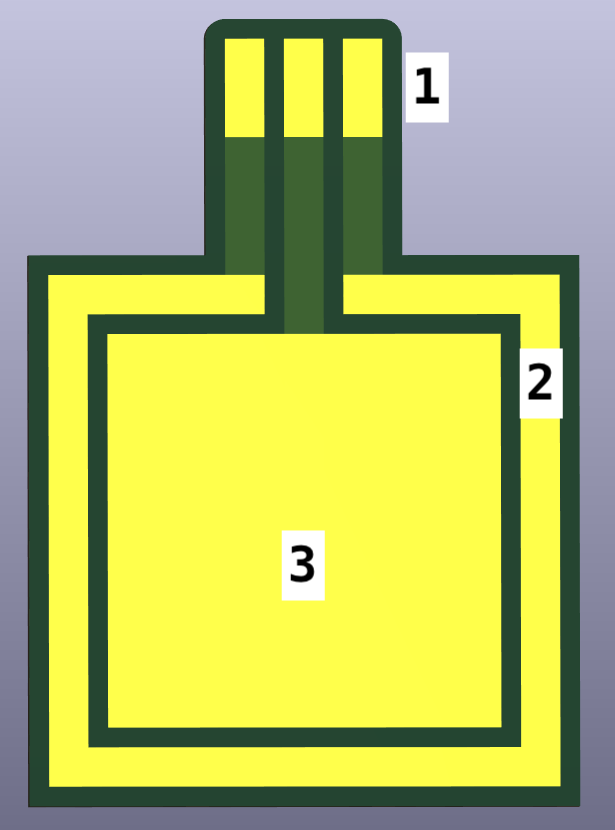
\includegraphics[width=0.5\textwidth]{Figures/GoldElectrode}
    \caption{The gold electrode \gls{pcb} design.}
    \label{fig:gold-electrode} %chktex 24
\end{figure}

The titanium electrodes are substantially simpler and cheaper than the gold electrodes and would be the preferred electrodes if the fringing effect could be accounted for.
Provided the testing with the gold electrodes is able to prove a constant resistance-voltage relationship, the fringing effect between the titanium electrodes could be measured and accounted for allowing for them to be used as the primary electrodes in a future iteration of the device.
The titanium wire that was available for this project was $1mm$ in diameter and in order to account for the unknown resistance between the electrodes, the design allowed for an adjustable spacing between the electrodes and adjustable electrode length.

\subsection{Conductivity Measurement and Calibration}

The conductivity measurement is done by measuring the resistance of the water between the two electrodes and performing a calculation to convert this to a conductivity value.
The most common and practical method of measuring resistance is to use a resistor divider circuit and measure the voltage across the water.

As electrical fringing is a problem in conductive materials such as salt water and increase exponentially with voltage, this device aimed to keep the voltage across the water low.
This was achieved by aiming for a resistor divider with R1 around 10 times greater than R2 which would be the salt water.
The voltage of the voltage divider was then amplified by a factor of 10 to increase the resolution of the measurement.

A distibuted factor about salt water is whether its resistivity is constant or not.
To determine this, the resistor divider was powered using a DAC which would allow for the voltage across the water to be varied and the resistance to voltage fit could be calculated.

To account for certain uncertainties of the design such as the resistance between the titanium electrodes, the resistor R1 was given mutliple options which could be selected using solder jumpers in the device.

Additionally to combat the effects of fringing a fringe guard was added to the gold electrodes that would ideally take up all the fringing allowing for the resistance measurement to be completely accurate.
\textit{fringe guard image and calcs here}

\subsection{Accounting for Electrical Fringing}
fill from above

\subsection{Accounting for Unkown Resistivity of Salt Water}
fill from above

\subsection{Salinity Calculation and Display}
The salinity probe was requried to be lowered into the water and the salinity to be measured.
The two options for capturing the salinity were to either record the data and write it to an SD card which would create problems with waterproofing the device and making the SD card accessible.
The alternative was to have a probe that communicates with a controller where the controller would instruct the probe to take a measurement and then the probe would send the data back to the controller.
RS485 for coms.

\subsection{Temperature and Depth Measurement}

The depths sesnors that are waterproof are increadibly expensive which made them unfeasable for this project.
There have been alternative approaches which use non waterproof sensors that are isolated form the water using a flexible membrane that would allow the pressure to be transmitted to the sensor.

The temperature sensor used in this project was a XXX which was chosen for its accuracy and low cost.
The temperature sensor must be close to the water to prevent the low thermal conductivity of the epoxy resin from affecting the temperature measurement.
Additionally the STM was powerful enough to include its own temperature sensor.

\subsection{Controller and Data Logging}
\textit{waterproofing device}

\section{Device Coding}
ur mom

